\subsection{Results for Co-discovery}
The functionality primarily used while trying to solve the assignments was the main search bar, located at the top center, see \autoref{results:amazonsearchbar}. As well as the sorting function of the found results for a given search, sorted primarily by price, see \autoref{results:amazonsortby}.

\begin{figure}[h]

\includegraphics[scale=0.3]{./includes/amazon_search_bar.png}
\label{results:amazonsearchbar}
\caption{Amazon main search bar}
\end{figure}

\begin{figure}[h]
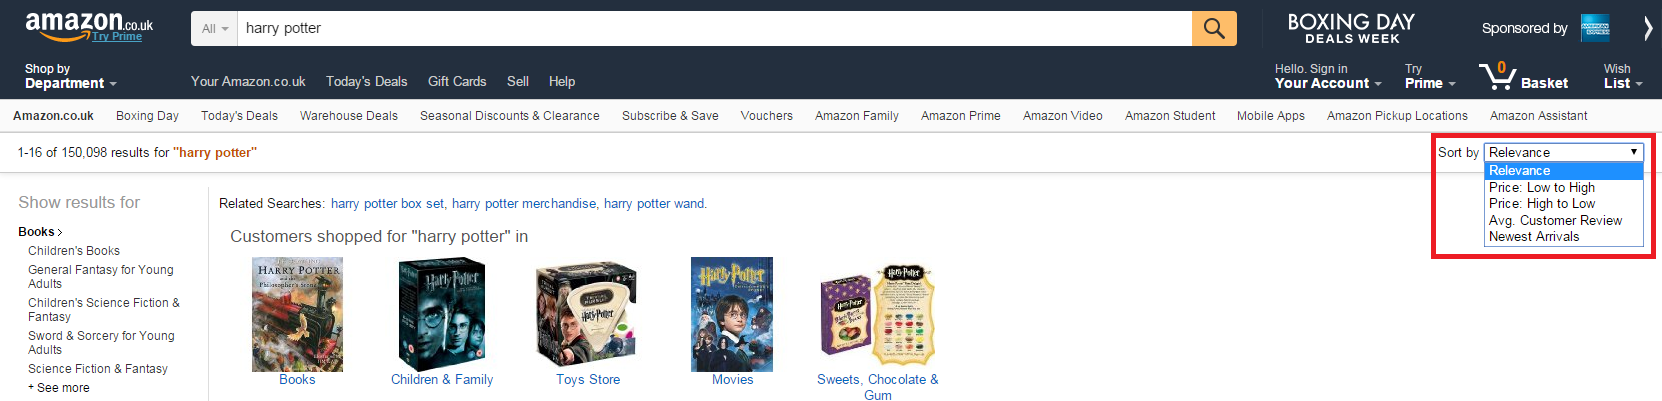
\includegraphics[scale=0.3]{./includes/amazon_sort_by.png}
\label{results:amazonsortby}
\caption{Amazon sort search result by}
\end{figure}
\bjarke{find tool to highlight important parts of pictures}

The functionality that we considered useful, and expected to be used, included the recommender system, and the category drop-down menu in the top left corner, which were never utilized, see \bjarke{insert pics}. Also the participants became rather confused when trying to find the relevant information regarding shipping of a certain product.

\subsection{Results for AttrakDiff}
The results of the AttrakDiff can be seen in ... below. \\

\bjarke{lav figur med resultater} \\

From the results of the AttrakDiff questionare we observed that the participants agreed that the system was
\begin{itemize}
\item Simple
\item Easy to use
\item Practical
\item Professional
\end{itemize}
However they didn't find it especially:
\begin{itemize}
\item Social
\item Innovative
\item Creative
\item New
\end{itemize}